\title{Архитектура интерпретатора\\ 
для исполнения программ на языке PostScript\\
в JVM}
%
\titlerunning{Архитектура интерпретатора PostScript}
\author{Макулов Рустам Наилевич}
%
\authorrunning{Р.Н.Макулов} % abbreviated author list (for running head)
%
%%%% list of authors for the TOC (use if author list has to be modified)
\tocauthor{Р.Н.Макулов}
%
\institute{Санкт-Петербургский государственный университет\\
\email{r.n.makulov@gmail.com}}

\maketitle              % typeset the title of the contribution

\begin{abstract}
На сегодняшний день многие языки программирования имеют реализации, использующие в качестве среды выполнения 
виртуальную машину Java. Данная работа выполнялась в рамках проекта по разработке переносимого интерпретатора языка PostScript. 
Для интерпретатора такого богатого языка принципиально важным является решение проблемы разработки его архитектуры~--- декомпозиции 
на компоненты, адекватное представление данных, учитывая, что одной из нестандартных интересных возможностей языка PostScript 
является наличие примитивов сохранения/восстановления состояния локальной памяти. Разработке такой архитектуры и представления 
данных была посвящена данная работа.
\end{abstract}

\section*{Введение}

Одной из задач программной инженерии является создание средств, позволяющих сделать процесс разработки более простым, удобным и универсальным. Все больше внимания уделяется кроссплатформенности программ, при которой программное обеспечение (ПО), написанное один раз, поддерживается более чем одной аппаратной платформой или операционной системой. Можно выделить два типа такого ПО: первый тип требует отдельной сборки или компиляции для каждой поддерживаемой платформы, а второй – может быть непосредственно запущен на любой платформе без предварительной подготовки. Ко второму типу относятся программы, написанные на интерпретируемом языке или предварительно скомпилированные в байт-код. Для них интерпретатор или среда исполнения являются общей или стандартной компонентой многих платформ. В целом это упрощает процесс разработки и делает его более универсальным с точки зрения перенесения с одной платформы на другую.
Для реализации ПО второго типа применяются виртуальные машины. Они исполняют некоторый машинно-независимый код или машинный код реального процессора. Одной из виртуальных машин, предназначенных для исполнения байт-кода, является виртуальная машина Java (JVM)\cite{jvms}.

JVM первоначально была разработана для поддержки только языка программирования Java. Тем не менее, с течением времени все больше языков были адаптированы или созданы  для работы на Java-платформе. Например, исходный код на языке Ada\footnote{\url{http://www.adacore.com/press/ada-java\_interfacing\_suite}} может быть откомпилирован в байт-код Java, который затем можно выполнить с помощью JVM. Помимо Ada, многие существующие языки имеют JVM-реализации, например, C\footnote{\url{http://nestedvm.ibex.org/}}, Cobol\footnote{\url{http://www.elasticcobol.com/}}, Common Lisp\footnote{\url{http://clforjava.org/}}, Erlang\footnote{\url{http://erjang.org/}}, JavaScript\footnote{\url{http://www.mozilla.org/rhino}}, OCaml\footnote{\url{http://ocamljava.x9c.fr/}}, R\footnote{\url{http://code.google.com/p/renjin/}}, Ruby\footnote{\url{http://jruby.org/}} и так далее. Таким образом, JVM является универсальной платформой для исполнения программ на многих языках программирования. 

Данная работа посвящена разработке архитектуры переносимого интерпретатора программ на языке PostScript \cite{plrm} в JVM-среде. PostScript —  это гибкий,  компактный и мощный язык	программирования, предназначенный как для отображения графических изображений, так и для выполнения других задач программирования. Как и в случае со многими языками, PostScript был разработан для конкретной цели – для описания сложной цифровой графики аппаратно-независимым образом. Несмотря на легкость в изучении, программы на этом языке генерируются в основном другими программами. Результат выполнения PostScript-программ может быть показан на экране в виде документа. Для выполнения программ, написанных на PostScript, существуют интерпретаторы языка для каждой  операционной системы.
В рамках работы решается задача построения и реализации архитектуры интерпретатора для исполнения программ на языке PostScript в среде виртуальной машины Java. Для этого необходимо спроектировать и реализовать модель памяти языка, иерархию объектов, структуры данных.

\section{Общие сведения о языке PostScript}
PostScript --- это полнофункциональный тьюринг-полный язык программирования. Синтаксис языка использует обратную польскую нотацию. Далее мы рассмотрим используемую в языке модель данных и основные компоненты среды исполнения.

\subsection{Модель данных}
Все данные, доступные программам на PostScript, включая процедуры, существуют в виде объектов. Они вызываются и управляются  PostScript-операторами. 

Каждый объект имеет значение, тип и атрибуты. Атрибуты влияют на поведение объектов во время их исполнения или выполнения над ними определенных операций, но не при непосредственном рассмотрении их в качестве данных. Например, два целых числа считаются равными, даже если у них разные атрибуты.

Объекты бывают простые, например: boolean, integer, real, name, mark, null и сложные, например: array, dictionary, file, string, file. Про некоторые из них нужно сказать отдельно.
\begin{itemize}
\item Именованные объекты (name) используются как идентификаторы в других языках программирования: теги для переменных, процедур и так далее. При этом в языке можно определить именованный объект без привязки к какому-либо объекту.
\item Словари (dictionary) представляют собой ассоциативный массив, элементами которого является пара PostScript-объектов. Первый из них ключ, второй -- значение. В качестве ключей обычно выступают именованные объекты.
\item Массивы в языке могут включать объекты разного типа. Если в атрибутах массива указано, что он исполняемый, то он является процедурой.
\item Метки (mark) -- специальные объекты, служащие для обозначения позиции на стеке операндов. Они используются, например, при ручном вводе элементов массива: сначала на стек операндов кладется метка, затем поочередно элементы. Когда ввод окончен, до тех пор пока не дойдут до метки, из стека достаются элементы. В итоге на стек операндов кладется один единственный массив со всеми его элементами. Строки и словари также имеют свои метки.
\end{itemize}

Большинство объектов являются простыми. Они являются неделимыми: их тип, значение и атрибуты неизменно связаны друг с другом и не могут быть изменены. В отличие от простых объектов значение сложных объектов отделено от самих объектов. Некоторые сложные типы имеют внутреннюю видимую структуру и могут быть частично изменены.

Отличие простых объектов от сложных заключается в их поведении при операции копирования. Копирование – это любая операция, которая передает содержимое объекта из одного места памяти в другое. Примерами таких операций является выборка и сохранение. Можно получать новый объект, копируя существующий с некоторыми изменениями.

Когда происходит копирование простого объекта, все его части (тип, атрибуты и значение) копируются вместе. Когда происходит копирование сложного объекта, значение не копируется; вместо этого исходный и скопированный объекты разделяют одно значение.  Поэтому любые изменения, внесенные в структуру значения одного объекта, также проявляются в части значения другого объекта.

Разделение значений сложных объектов в языке PostScript соответствует использованию указателей в таких языках как C и Pascal. В действительности, интерпретатор языка PostScript использует указатели для реализации разделяемых значений; сложные объекты содержат ссылки на свое значение. Тем не менее, в языке PostScript отсутствует явное понятие указателя.


\subsection{Виртуальная память}

Значения простых объектов содержатся в них самих. Значения сложных объектов располагаются в специальной области памяти, которая называется виртуальной памятью. Виртуальная память разделена на локальную и глобальную. По умолчанию установлен локальный режим выделения памяти. Переключение на выделение места в глобальной памяти производится при помощи оператора setglobal.

Локальную память можно рассматривать в качестве специальной области памяти, над которой работают операторы save и restore. Значения расположенных в ней объектов сохраняются и восстанавливаются при помощи этих операторов. Использование данных операторов вводит структурность программы. Поэтому в программах локальная память чаще всего используется для хранения информации, которая соответствует только определенной структурной единице и потом не нужна --- например, на одной странице.  Глобальная память используется для хранения информации, время жизни которой не зависит от структуры, --- ресурсов, подгружаемых динамически во время выполнения.


\subsection{Стеки}

В PostScript для хранения данных разного типа используются следующие стеки: стек операндов, стек словарей, стек графических состояний и стек исполнения. 
\begin{itemize}
\item В стеке операндов хранятся произвольные объекты языка. Они могут быть как операндами, так и результатом работы PostScript-операторов. Объекты кладутся на стек операндов только тогда, когда рассматриваются интерпретатором в качестве данных, но не в качестве исполняемых объектов.
\item 	В стеке словарей хранятся только словари. Набор этих словарей определяет неявную среду для поиска имен, среди которых интерпретатор ищет очередной исполняемый именованный объект.
\item 	В стеке исполнения хранятся исполняемые объекты (в основном процедуры и файлы), которые находятся в стадии исполнения. В любой точке исполнения программы он представляет собой стек вызовов программы.
\item 	Стек графических состояний используется для хранения полных копий графического состояния, сделанных оператором gsave. Они используются при восстановлении графического состояния оператором grestore.
\end{itemize}


\subsection{Операторы save и restore}
Операторы save и restore используются для сохранения и восстановления значения объектов в локальной памяти. Оператор save сохраняет состояние локальной памяти и возвращает сохраненное состояние. Оператор restore возвращает состояние локальной памяти к состоянию, сохраненному предшествующим оператором save. Более точно, restore делает следующее:
\begin{itemize}
\item освобождает локальную память от значений всех объектов, которые были созданы с момента соответствующей операции save;
\item восстанавливает значения всех сложных объектов в локальной памяти, кроме строк, к их состоянию на момент операции save;
\item выполняет неявную операцию grestoreall, которая возвращает значение графического состояния к значению на момент операции save;
\item закрывает файлы, которые были открыты после соответствующей операции save в локальной памяти.
\end{itemize}

Операция restore согласно спецификации не должна производить следующие действия:
\begin{itemize}
\item изменять содержимое стека операндов, стека словарей и стека исполнения; 
\item изменять любые объекты, расположенные в глобальной памяти;
\item отменять побочные эффекты за пределами виртуальной памяти, такие как вывод данных в файл или отображение графики на растровом устройстве вывода; тем не менее оператор grestoreall способен отключить текущее устройство, тем самым стирая текущую страницу.
\end{itemize}

Операторы save и restore могут быть вложены ограниченное число раз. Программы на языке PostScript могут использовать эти операторы для инкапсуляции исполнения встроенных программ, в которых они также могут использоваться.
Существуют специальные соглашения, в которых описан вид специальных структурных программ, описывающих страницы. Для таких программ операторы save и restore выполняют в следующих целях.
\begin{itemize}
\item Документ состоит из пролога и скрипта. Пролог содержит определения, которые используются во всем документе. Скрипт содержит последовательность независимых страниц. В начале каждой вызывается оператор save, и оператор restore – в конце, непосредственно перед оператором отображения showpage. Каждая страница начинается с возвращения локальной памяти к начальному состоянию, установленному прологом. Таким образом, отсутствуют нежелательные эффекты с предыдущих страниц.
\item Некоторые страницы содержат дополнительные конструкции, например встроенные картинки, исполнение которых тоже должно быть инкапсулировано. Инкапсулированная программа для каких-то своих задач может внести много изменений в содержимое локальной памяти. Поместив программу между save и restore, объемлющая программа  изолируется от результатов работы встроенной программы.
\item По мере выполнения программы на PostScript в локальной памяти накапливаются новые сложные объекты. Оператор restore восстанавливает всю локальную память, выделенную с момента соответствующего снимка; периодическое выполнение операций save и restore гарантирует, что невостребованные объекты не исчерпают все доступные ресурсы локальной памяти. В первой версии языка PostScript эти операции были единственным способом восстановления локальной памяти. Даже в новых версиях языка этот способ гораздо более эффективен, чем автоматическая сборка мусора.
\item Интерпретатор языка PostScript использует операции save и restore для инкапсуляции исполнения индивидуальных заданий в контексте использования интерпретатора в специальном окружении.
\end{itemize}

Для того, чтобы в глобальной памяти после операции restore не появлялись ссылки на несуществующие объекты в локальной памяти, ссылки на такие объекты запрещены. При попытке сохранения локального объекта в качестве элемента глобального возникает ошибка.


\subsection{Примеры использования операторов save и restore}

Для примера возьмем несколько простых программ на PostScript для демонстрации некоторых особенностей языка. 


%\begin{figure} [h]
%\caption{Простой объект на стеке операндов после операции save}
\begin{lstlisting}[label=PostScript-example3,caption=Простой объект на стеке операндов после операции save, language = PostScript]
/AnArray 10 array def
AnArray
save
7
exch
restore
\end{lstlisting}
%\end{figure}

В первой строке заводится массив на 10 элементов и кладется на стек операндов во второй строке. В третьей строке выполняется сохранение состояния локальной памяти. В четвертой строке на стек операндов кладется число семь. Теперь на стеке 3 объекта: внизу массив, выше снимок локальной памяти и наверху новое число. В пятой строке меняются местами два верхних элемента стека --- для корректного восстановления состояния локальной памяти в шестой строке. Число, созданное после операции save, остается на стеке.


%\begin{figure} [h]
%\caption{Сложный объект на стеке операндов после операции save}
\begin{lstlisting}[label=PostScript-example4,caption=Сложный объект на стеке операндов после операции save, language = PostScript]
save
/AnArray 10 array def
AnArray
restore
\end{lstlisting}
%\end{figure}

В первой строке выполняется сохранение состояния локальной памяти. Во второй строке заводится массив на 10 элементов и кладется на стек операндов в третьей строке. В четвертой строке вызывается оператор restore, но возникает ошибка: на стеке операндов сложный объект, созданный после сохранения состояния. Локальная память не восстановлена.


%\begin{figure} [h]
%\caption{Изменение значения строки}
\begin{lstlisting}[label=PostScript-example1,caption=Изменение значения строки, language = PostScript]
/str (String) def 		% (String)
str 1 (test) putinterval	% (Stestg)
save
str 1 (trin) putinterval	% (String)
restore				% (String)
\end{lstlisting}
%\end{figure}


В первой строке создается строка str. Во второй строке производится замена подстроки строки str на строку со значением test начиная с первого символа.  В третьей строке выполняется операция save --- на стек операндов кладется снимок состояния локальной памяти. В четвертой строке производится замена подстроки строки str на строку со значением trin, начиная с первого символа. В итоге, в пятой строке после операции restore исходное значение строки str не восстанавливается: ее значение не вернулось к тому, что было во время операции save. 


%\begin{figure} [h]
%\caption{Изменение значения массива}
\begin{lstlisting}[label=PostScript-example2,caption=Изменение значения массива, language = PostScript]
/AnArray 10 array def		% [null null null null null null null null null null]
AnArray 8 (str) put		% [null null null null null null null null (str) null]
save
AnArray 8 (tst) put		% [null null null null null null null null (tst) null]
restore				% [null null null null null null null null (str) null]
\end{lstlisting}
%\end{figure}


В первой строке заводится массив на 10 элементов. По умолчанию все элементы null. Во второй строке элемент под номером восемь изменяется на строку str.  В третьей строке выполняется операция save --- на стек операндов кладется снимок состояния локальной памяти. В четвертой строке элемент под номером восемь заменяется на строку tst. В итоге, в пятой строке после операции restore исходное значение элемента массива восстанавливается: на месте восьмого элемента снова строка str. 

Два последних примера показывают некую неоднозначность в работе данных операторов. С одной стороны, согласно спецификации строки не подлежат восстановлению, но с другой стороны, согласно той же спецификации, если они хранятся в качестве значения какого-то другого объекта, то их значение восстанавливается к исходному перед сохранением.

\subsection{Сборка мусора}
Помимо ручного освобождения места в памяти, в языке PostScript предусмотрена автоматическая сборка мусора. Сборщик мусора очищает память от объектов, которые более недоступны программе. Например, это могут быть какие-то элементы старых значений сложных объектов.

Несмотря на сборку мусора операторы save и restore не меняют своего поведения. restore восстанавливает все доступные объекты в локальной памяти к моменту операции save. Все объекты, созданные в локальной памяти после операции save, удаляются, при этом затрачивается намного меньше ресурсов. Но с другой стороны, сборка мусора --- это единственный способ очистки глобальной памяти, так как save и restore не затрагивают её.


\section{Архитектура интерпретатора}
С точки зрения языка Java архитектура --- это иерархия объектов, которая достаточно полно описывает все объекты языка, а также основные компоненты среды исполнения: виртуальную память и необходимые стеки. 

\subsection{Виртуальная память}
Внутреннее представление интерпретатора реализовано в классе Runtime. Этот класс содержит в себе в качестве полей объекты классов LocalVM, OperandStack, DictionaryStack, GraphicStack и CallStack, которые реализуют локальную память, стек операндов, стек словарей, графический стек и стек вызовов языка PostScript соответственно.

Локальная память предназначена только для хранения значений сложных объектов. Для реализации операций сохранения и восстановления состояний локальной памяти в интерпретаторе применена двухуровневая адресация, то есть сложные объекты вместо своего значения содержат ссылку на него. Благодаря этому во время операции восстановления меняется не объект, а его значение по ссылке. С этой же целью все объекты сделаны неизменяемыми --- при попытке внесения в них изменений создается новый объект. Таким образом, если изменить локальный объект после сохранения состояния, сохраненное значение не изменится.

Локальная память в интерпретаторе реализована в виде класса LocalVM. Его основной компонент --- объект класса Map является хранилищем значений сложных объектов. В качестве ключа используется ссылка на объект, а в качестве значения возвращается значение объекта. Значения в память добавляются при помощи метода add(). Этот метод возвращает ссылку на переданное ему значение в памяти. Метод setValueAtIndex() данного класса использует ссылки, чтобы при необходимости обновить значение по адресу ссылки. Таким образом, при операции restore достаточно подменить значение по ссылке в локальной памяти, не нужно менять сами объекты.

Объекты, создаваемые в глобальной памяти, интерпретатор размещает в памяти JVM. Они не входят в область действия операторов save и restore, и поэтому могут быть удалены только сборщиком мусора.

Переключение между двумя типами памяти производится при помощи метода setGlobal() в классе Runtime.

\begin{figure}[t]
\center{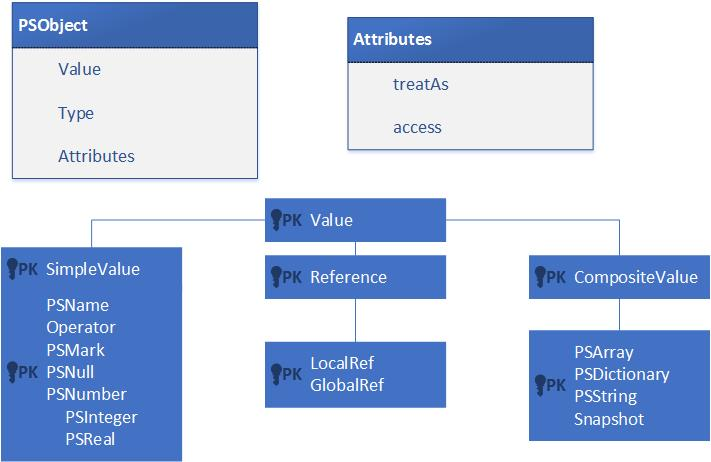
\includegraphics[width=\linewidth]{Makulov/class_diagram.jpg}}
\caption{Диаграмма классов}\label{pic_Frame}
\end{figure}

\subsection{Иерархия объектов}

Каждый объект языка PostScript реализован в виде класса PSObject. Он имеет три поля: значение, тип и атрибуты (рис.~\ref{pic_Frame}). Значение всех объектов наследуется от абстрактного класса Value, в котором есть абстрактный метод getValue(). Для простых значений он возвращает этот же простой объект, для сложных -- используя ссылку, значение сложного объекта в локальной памяти. 

\begin{itemize}
\item SimpleValue ---  базовый абстрактный класс, объединяющий все значения простых объектов.
\item CompositeValue --- базовый абстрактный класс, объединяющий все значение сложных объектов. Объекты данного класса доступны только по ссылке.
\item Reference --- базовый абстрактный класс, представляющий собой ссылку на значение сложного объекта. Имеет два абстрактных метода getValue() и setCompositeValue(). Последний метод меняет значение и возвращает один из атрибутов присвоенного объекта, а именно его тип.
\item LocalRef ---  класс, представляющий собой ссылку на значение сложного объекта в локальной памяти. Метод setCompositeValue() позволяет заменить значение, которое лежит по адресу в этой ссылке.
\item GlobalRef ---  класс, представляющий собой ссылку на сложный объект в глобальной памяти. Метод setCompositeValue() заменяет значение, лежащее внутри этой ссылки.
\item PSNumber --- абстрактный класс, представляющий собой все числа языка.
\item PSInteger --- класс, представляющий собой целые числа языка.
\item PSReal --- класс, представляющий собой вещественные числа языка.
\item PSName ---  класс, представляющий собой именованные объекты в языке.
\item Operator --- базовый абстрактный класс, от которого наследуются все операторы языка. Имеет абстрактный метод execute(), который реализован в каждом операторе согласно назначению каждого.
\item PSMark ---  класс, представляющий собой метки в языке. Поддерживаются все типы меток.
\item PSBoolean ---  класс, представляющий собой логические константы в языке.
\item PSNull ---  класс, представляющий собой пустые объекты в языке.
\item PSDictionary ---  класс, представляющий собой словари. Они реализованы в виде AVL-дерева.
\item PSString ---  класс, представляющий собой строки в языке. Реализован в виде массива из объектов класса StringElement. В языке каждый элемент строки рассматривается отдельно и кодируется некоторым числом, поэтому класс StringElement хранит в себе некоторое число, которое можно получить при помощи метода getCharacter() и изменить при помощи метода setCharacter().
\item PSArray ---  класс, представляющий собой массивы в языке. Реализован в виде массива из объектов класса ArrayElement, каждый их которых хранит в себе отдельный объект класса PSObject, которые можно получить и изменить аналогично элементам строк.
\item Snapshot ---  класс, представляющий собой снимки состояния локальной памяти. Хранит в себе копию локальной памяти на определенный момент времени.
\item Attribute --- класс, отвечающий за атрибуты объекта. В качестве полей содержит объекты двух перечисляемых типов: Access и TreatAs. Доступ может быть неограниченным, только для чтения, только для исполнения и закрыт; объект может рассматриваться как исполнимый, либо как данные.
\end{itemize}

Все объекты могут быть сравнимы между собой и поэтому в каждом классе реализованы методы compareTo() и equals().

\subsection{Значения объектов и операторы save и restore}

Значения всех объектов сделаны неизменяемыми. Объекты могут изменить свое значение только в том случае, если они сложные. В этом случае  подменяется значение, которое лежит по ссылке (Reference). Если ссылка локальная, то по адресу этой ссылки в локальной памяти значение меняется на новое. При изменении объекта, содержащего ссылку на глобальную память, подменяется значение, которое находилось в этой ссылке в качестве поля. Поскольку все значения неизменяемые или immutable, то все методы, их изменяющие, возвращают новые изменённые значения. Старые значения либо используются по-прежнему используются другими объектами, либо удаляются сборщиком мусора.

Операторы save и restore реализованы в классе Runtime. Оператор save делает копию локальной памяти и кладет ее на вершину стека операндов. Оператор restore берет объект с вершины стека операндов и проверяет, является ли данный объект снимком состояния памяти. Далее берется каждый элемент стека операндов и, если это сложный объект, который был создан после операции save (т.е. его нет в снимке памяти), выбрасывается ошибка, операция restore не выполняется. Если ошибок не возникло, то обновляется значение всех строк из снимка (restore не меняет значения строк согласно спецификации). В конце локальная память возвращается к состоянию на обновленном снимке. 

\section*{Заключение}

В рамках данной работы построена и реализована архитектура для интерпретатора программ на языке Postscript. Реализованная архитектура правильным образом описывает все основные компоненты: локальную и глобальную память, стек операндов, стек словарей, стек исполнения и графический стек. Реализована иерархия объектов, поддерживаются операторы сохранения состояния локальной памяти, для сохранения состояния локальной памяти все объекты неизменяемые, среда исполнения реализована на Java. Есть тестовая база, которая работает как в эталонном интерпретаторе ghostscript.

\begin{thebibliography}{99}
\bibitem{jvms}
Tim Lindholm, Frank Yellin, Gilad Bracha, Alex Buckley.
The Java Virtual Machine Specification.
Java SE 8 Edition, 2014. \\
\url{http://docs.oracle.com/javase/specs/jvms/se8/html/}

\bibitem{plrm}
PostScript Language Reference, Third Edition, 1999, 912 p. \\
\url{http://www.adobe.com/products/postscript/pdfs/PLRM.pdf}
\end{thebibliography}
